\documentclass[11pt,a4paper]{article}
\usepackage{listings}
\usepackage{a4wide}
\usepackage{amsmath}
\usepackage{amssymb}
\usepackage{amsfonts}
\usepackage{verbatim}
\usepackage{fancyvrb}
\usepackage{fixltx2e}
\usepackage[utf8]{inputenc}
%\usepackage[latin1]{inputenc}
\usepackage[T1]{fontenc}
\usepackage[spanish]{babel}
\usepackage{indentfirst}
\usepackage{fancyhdr}
\usepackage{latexsym}
\usepackage{lastpage}
\usepackage{caratula}
\usepackage[colorlinks=true, linkcolor=black]{hyperref}
\usepackage{calc}
\usepackage{alltt}
\usepackage{verbatim}
\usepackage{caption}
\usepackage{hyperref}
\usepackage{url}
\usepackage{graphicx, subfigure}
\usepackage{float}
\usepackage{algorithm}
\usepackage{algorithmic}
\floatname{algorithm}{Algoritmo}
\renewcommand{\listalgorithmname}{Lista de algoritmos}
\renewcommand{\algorithmicrequire}{\textbf{Entrada:}}
\renewcommand{\algorithmicensure}{\textbf{Salida:}}
\renewcommand{\algorithmicend}{\textbf{fin}}
\renewcommand{\algorithmicif}{\textbf{si}}
\renewcommand{\algorithmicthen}{\textbf{entonces}}
\renewcommand{\algorithmicelse}{\textbf{si no}}
\renewcommand{\algorithmicelsif}{\algorithmicelse,\ \algorithmicif}
\renewcommand{\algorithmicendif}{\algorithmicend\ \algorithmicif}
\renewcommand{\algorithmicfor}{\textbf{para}}
\renewcommand{\algorithmicto}{\textbf{hasta}}
\renewcommand{\algorithmicforall}{\textbf{para todo}}
\renewcommand{\algorithmicdo}{\textbf{hacer}}
\renewcommand{\algorithmicendfor}{\algorithmicend\ \algorithmicfor}
\renewcommand{\algorithmicwhile}{\textbf{mientras}}
\renewcommand{\algorithmicendwhile}{\algorithmicend\ \algorithmicwhile}
\renewcommand{\algorithmicloop}{\textbf{repetir}}
\renewcommand{\algorithmicendloop}{\algorithmicend\ \algorithmicloop}
\renewcommand{\algorithmicrepeat}{\textbf{repetir}}
\renewcommand{\algorithmicuntil}{\textbf{hasta que}}
\renewcommand{\algorithmicprint}{\textbf{imprimir}} 
\renewcommand{\algorithmicreturn}{\textbf{devolver}} 
\renewcommand{\algorithmictrue}{\textbf{cierto }} 
\renewcommand{\algorithmicfalse}{\textbf{falso }} 

\parskip = 11pt

% Pseudocódigo a lo Cormen
\usepackage{package/clrscode}

% auxiliares
\newcommand{\sisosi}{\Leftrightarrow}

\newcommand{\Frac}{\displaystyle\frac}

\newcommand{\suma}[2]{\sum\limits_{#1}^{#2}}

\newcommand{\Suma}[2]{\displaystyle\sum\limits_{#1}^{#2}}

\newcommand{\bc}{\begin{center}}
\newcommand{\ec}{\end{center}}


%\addtolength{\hoffset}{-1cm}
%\addtolength{\textwidth}{2cm}
 \addtolength{\voffset}{-0.5cm}
 \addtolength{\textheight}{1cm}
 
 %Datos de la caratula
\materia{Algorítmos y Estructura de Datos III}
\subtitulo{Algoritmos, complejidad, recursión}
\titulo{Reentrega Trabajo Práctico 2}

\fecha{07 / 10 / 2014}
\integrante{Augusto Mascitti}{954/11}{mascittija@gmail.com}
\integrante{Patricio Capanna}{866/10}{patriciocapanna@gmail.com}
\integrante{Ariel Paez}{668/09}{twizt.hl@gmail.com}


\newcommand{\real}{\mathbb{R}}
\newcommand{\nat}{\mathbb{N}}
\newcommand{\eme}{\mathcal{M}}
\newcommand{\emeh}{\widehat{\mathcal{M}}}
\newcommand{\ere}{\mathcal{R}}

%%%%%%%%% MACROS %%%%%%%%%
\urldef\wikiMakefile\url{http://es.wikipedia.org/wiki/Make}
\urldef\mnistURL\url{http://yann.lecun.com/exdb/mnist/}
\urldef\wikiHouseholder\url{http://en.wikipedia.org/wiki/QR_decomposition#Using_Householder_reflections}

%%%%%%%% FIN MACROS %%%%%%

\parskip=5pt % 10pt es el tama�o de fuente

\begin{document}

\thispagestyle{empty}
\maketitle
\tableofcontents



\newpage
\section{Problema 1: Plan de Vuelo}
\subsection{Descripci\'on del problema}

\noindent
Somos parte del equipo de desarrollo de una web de ventas de pasajes aereos, y queremos ofrecerles a nuestros clientes un servicio que le calcule el itinerario mediante el cual puede llegar de una ciudad, a otra.Se quiere que el itinerario calculado llegue al destino en el menor tiempo posible. Para esto debe evaluar todos los trasbordos necesarios para que el momento de llegada sea minimo. \\
Hay una restriccion que dee cumplirse, en un trasbordo, tiene que haber por lo menos dos horas de diferencia entre la hora de llegada a la ciudad, hasta la salida del proximo vuelo. \\

\subsection{Resoluci\'on}

\noindent
Para resolverlo interpretamos la entrada como un grafo dirigido donde cada ciudad es un vertice, y donde las aristas son los viajes disponibles de una ciudad a otra. \\
Las aristas se definen dinamicamente en el grafo y tienen un costo asociado, correspondiente al costo temporal de viajar de la ciudad $X$ a la ciudad $Y$ m\'as el tiempo de espera desde arrivado a la ciudad $A$.

\noindent
Qu\'e queremos decir con que las aristas se definen dinamicamente?  \\
Empezamos por identificar que el problema es b\'asicamente encontrar un camino m\'inimo entre la ciudad A y B. Pero no podemos simplemente utilizar un algoritmo que resuelva el camino m\'inimo entre esos dos vertices ya que en principio no estamos seguros cuales son las aristas en el grafo. \\

\noindent
Decidimos implementar un Dijkstra modificado que busque el cam\'ino m\'inimo entre dos puntos de un grafo pero tal que vaya completando las aristas entre cada ciertos dos nodos seg\'un los nececite. \\

\noindent
Como resolvemos cuales son las aristas del grafo? \\
Para identificar una arista vamos a tener en cuenta dos cosas: \\
1- Para poder viajar de una ciudad X a una ciudad Y, debe haber una opci\'on de vuelo de X a Y y la hora de arrivo a X debe ser por lo menos 2 horas menor a la hora de salida de la opci\'on de vuelo o X es la ciudad de origen A.\\
2- Si hay m\'as de una opci\'on de vuelo entre una ciudad X y otra ciudad Y, y m\'as de una cumplen el item anterior (1), consideramos tomar como arista la que llegue a Y m\'as temprano. Si llego m\'as temprano a Y tengo igual o m\'as opciones de viaje para el vuelo siguiente. \\

\noindent
Dado un vertice origen, el algoritmo de Dijkstra reutiliza los caminos m\'inimos que ya calcul\'o para calcular contra de vertices no agregados todav\'ia a la solucion. El algoritmo s\'olo se fija aquellas aristas que parten de un vertice del conjunto soluci\'on hacia un vertice que todav\'ia no se encuentre en la soluci\'on. De esta manera podemos adaptar el algoritmo para que incorpore nuevas aristas justo cuando agregue un vertice nuevo a la soluci\'on. Estas aristas por supuesto corresponden a todas las aristas desde el vertice nuevo agregado hacia otros vertices. \\
Para identificar cuales son las aristas nuevas desde el vertice nuevo agregado tenemos en cuenta (1), considerando que la m\'inima hora de arrivo a la ciudad Y es igual al costo del cam\'ino m\'inimo desde X hasta Y, y tenemos en cuenta (2) resultando siempre en definir la arista de menor costo posible.\\

\noindent
La soluci\'on al problema es finalmente el camino m\'inimo entra X e Y calculado por el algoritmo modificado de Dijkstra, que se sigue comportando como Dijkstra, s\'olo que define las aristas del grafo antes de consultar por ellas. \\
\bigskip
\bigskip

\noindent
La resoluci\'on del problema se divide en varias partes:

\begin{itemize}
\item Parsear entrada.
\item Aplicar dijkstraAutofill para busqueda de camino minimo.
\item Obtener solucion del resultado de dijkstra.
\end{itemize}

\noindent
$\proc{Parsear entrada}$ \\

Parseamos la entrada teniendo en cuenta las siguientes estructuras:

\begin{lstlisting}

struct Vuelo{
	Vuelo(int id, int idCiudadOrigen, int idCiudadDestino, Horario inicio, Horario fin);
	int id;
	int idCiudadOrigen, idCiudadDestino;
	Horario inicio, fin;
};

struct Ciudad{
	Ciudad(int id, string nombre);
	int id;
	string nombre;
	list<Vuelo> vuelos;
};

\end{lstlisting}
\bigskip

\noindent
La entrada se parsea un $vector<Ciudad>$, donde el indice es el id de la ciudad. Y el id de la ciudad se define por el orden en que est\'an en la entrada, desde $0$ incrementando en $1$ por cada nueva ciudad.\\
Por cada linea de la entrada se crea una o dos ciudades nuevas, si no existen todavia, y se agregan al vector de ciudades. Despu\'es se agrega el Vuelo que lo describe, a la Ciudad origen.\\
\bigskip

\noindent
pseudoc\'odigo de dijkstraAutofill: \\


\begin{itemize}
\item $\proc{DijkstraAutofill}$
\item V $:=$ $\{0,1,2,...,cantCiudades-1\}$, v $:=$ $0$
\item T $:=$ V - $\{v\}$, $\pi$(v) $:=$ $0$, pred(v) $:=$ $-$1 
\item (*) completar X con las aristas de v
\item $\textbf{para todo}$ u $\in$ V $\textbf{hacer}$
\begin{itemize}
	\item $\textbf{si}$ (v, u) $\in$ X $\textbf{entonces}$
	\begin{itemize}
		\item $\pi$(u) $:=$ costo(v, u), pred(u) $:=$ v
	\end{itemize}
	\item $\textbf{si no}$
	\begin{itemize}
		\item $\pi$(u) $:=$ $\infty$, pred(u) $:=$ $\infty$
	\end{itemize}
\end{itemize}
\item $\textbf{mientras}$ T $\neq$ $\varnothing$ $\textbf{hacer}$
\begin{itemize}
	\item elegir w $\notin$ T tal que $\pi$(w) = $min_{u \in T}$ $\pi$(u)
	\item $\textbf{si}$ no existe tal w 
	\begin{itemize}
		\item $\textbf{END}$
	\end{itemize}
	\item T $:=$ T $-$ w 
	\item (*) completar X con las aristas de w
	\item $\textbf{para todo}$ u $\in$ T y (w, u) $\in$ X $\textbf{hacer}$
	\begin{itemize}
		\item $\textbf{si}$ $\pi$(u) > $\pi$(w) + costo(w, u) $\textbf{entonces}$
		\begin{itemize}
			\item $\pi$(u) $:=$ $\pi$(w) + costo(w, u)
			\item pred(u) $:=$ w
		\end{itemize}
	\end{itemize}
\end{itemize}
\item $\textbf{devuelvo}$ pred
\end{itemize}
\bigskip

\noindent
Codigo de (*) completar X con las aristas de un vertice:

\begin{lstlisting}
void Dijkstra::completarAristas(Vertice v, int horarioLlegada){

  list<Vuelo>::iterator it;
  list<Vuelo>::iterator itIni = (*this->ciudades)[v].vuelos.begin();
  list<Vuelo>::iterator itFin = (*this->ciudades)[v].vuelos.end();
  for (it = itIni; it != itFin; it++){
    
    Vuelo vuelo = *it;
    if (horarioLlegada + 2 <= vuelo.inicio || horarioLlegada == 0){

      G[v][vuelo.idCiudadDestino].completa = true;

      int costo = vuelo.fin - horarioLlegada;
      if (costo < G[v][vuelo.idCiudadDestino].costo){
        G[v][vuelo.idCiudadDestino].id = vuelo.id;
        G[v][vuelo.idCiudadDestino].costo = costo;
      }
    }
  }
}
\end{lstlisting}

\noindent
Tal como explicamos anteriormente completa el grafo incluyendo las aristas de un vertice especifico, iterando sobre los vuelos de la ciudad correspondiente y eligiendo aquellos que representen menor costo y sean posibles de realizar. El horarioLlegada es el costo de llegar al vertice $v$, es decir la hora a la que se arriba a la ciudad que representa el vertice $v$.
\bigskip

\subsection{Complejidad del algoritmo}

Detallamos cada item por separado:

\begin{itemize}
\item Parsear entrada $O(n!)$
\item Aplicar dijkstraAutofill para busqueda de camino minimo $O(n^2)$
\item Obtener soluci\'on del resultado de dijkstra $O(n)$
\end{itemize}


\noindent
$\proc{Parsear entrada}$ \\
La complejidad es 2*O(buscarCiudad) + 2*(O(CrearCiudad)+ O(CrearVuelo)) = O(buscarCiudad) + O(CrearCiudad) + O(CrearVuelo)


\begin{lstlisting}

Vuelo::Vuelo(int id, int idCiudadOrigen, int idCiudadDestino, int inicio, int fin){
	this->id = id;
	this->idCiudadOrigen = idCiudadOrigen;
	this->idCiudadDestino = idCiudadDestino;
	this->inicio = inicio;
	this->fin = fin;
}

Ciudad::Ciudad(int id, string nombre){
	this->id = id;
	this->nombre = nombre;
}

\end{lstlisting}

\noindent
La complejidad de crear un vuelo es O(1) por ser una cantidad finita de operaciones y consultas de int.\\
La complejidad para ver si ya existe una ciudad es O(cantidadCiudades). La cantidadDeCiudades puede ir incrementando como m\'aximo en 2 por cada linea nueva. Y la cantidad de ciudades es como m\'aximo 2n+2.
El resultado es una complejidad de O(2n! + 2) = O(n!). \\
La complejidad de crear una ciudad es O(1+stringCopy), es decir de O(stringCopy). De acuerdo a lo comentado por la catedra rebajamos la complejidad a O(1).\\
La complejidad total luego es la suma de todas las complejidades anteriores = O(1) + O(n!) + O(1) = O(n!)
\bigskip

\noindent
$\proc{DijkstraAutofill}$ \\

\noindent
La Complejidad de dijkstraAutofill es la complejidad del algoritmo defecto de dijkstra m\'as la complejidad de completar las aristas. \\

\noindent
La complejidad de b\'usqueda de cami\'ino m\'inimo de dijkstra es por supuesto O($m^2$) donde m es la cantidad de ciudades. Dado que la cantidad de ciudades est\'a acotada como dijimos anteriormente por 2n+2. La complejidad resulta O($(2n+2)^2$) = O($n^2$) \\

\noindent
La complejidad de completar las aristas es, por cada llamada, recorrer los vuelos del vertice con el que se llama y realizar operaciones O(1) por cada uno. Siempre se llama con un vertice distinto y se hace 1 vez por cada vertice. Entonces la complejidad de esto es O(n).

\noindent
La complejidad total es O($n^2$) +  O($n$) =  O($n^2$)
\bigskip
\bigskip

\noindent
$\proc{Obtener Solucion}$ \\

\noindent
La complejidad es la de recorrer los predecesores de la ciudad destino hasta llegar al origen. C\'omo m\'aximo debe recorrer todas las m ciudades.  \\
Teniendo en cuenta como acotamos m anteriormente, el resultado es una complejidad es O(m) = O(n). 
\bigskip

\noindent
Finalmente la complejidad de todas las partes del algoritmo es O($n^2$). 



\subsection{C\'odigo fuente}

\noindent
C\'odigo de ej1.cpp:

\lstset{language=C++,
                basicstyle=\ttfamily\footnotesize,
                keywordstyle=\color{blue}\ttfamily,
                stringstyle=\color{red}\ttfamily,
                commentstyle=\color{green}\ttfamily,
                morecomment=[l][\color{magenta}]{\#},
                breaklines=true
}
\begin{lstlisting}

#include "ej1.h"

Ej1::Ej1(int idOrigen, unsigned int cantCiudades, vector<Ciudad> &ciudades){

	this->idOrigen = idOrigen;
	this->cantCiudades = cantCiudades;
	this->ciudades = ciudades;
	this->dijkstra = NULL;

}

double Ej1::resolverPlanDeVuelos(int idDestino){
	timespec ts_beg, ts_end;
	clock_gettime(CLOCK_PROCESS_CPUTIME_ID, &ts_beg);


	// BEGIN BIOHAZARD
	if (this->dijkstra == NULL)
		this->dijkstra = new Dijkstra(this->cantCiudades, this->idOrigen, &(this->ciudades));
	this->calcularSolucion(idDestino);
	this->mostrarSolucion();
	// END BIOHAZARD

	cout << "Tiempo de ejecucion: " << endl;
	clock_gettime(CLOCK_PROCESS_CPUTIME_ID, &ts_end);
	double time = (ts_end.tv_sec - ts_beg.tv_sec) + (ts_end.tv_nsec - ts_beg.tv_nsec) / 1e9;
	cout << time << " sec" << endl;
	cout << endl;

	return time;
}

void Ej1::calcularSolucion(int idDestino){

	list<int> vuelosTomados;
	int costoTotal = 0;
	Vertice vertice = idDestino;
	while (dijkstra->damePredecesor(vertice) != -1){
		Vertice predecesor = dijkstra->damePredecesor(vertice);
		vuelosTomados.push_front(this->dijkstra->dameIdArista(predecesor,vertice));
		costoTotal += this->dijkstra->dameCosto(predecesor,vertice);
		vertice = predecesor;
	}

	if (vertice == this->idOrigen){
		this->solucion = std::to_string(costoTotal) + " " + std::to_string(vuelosTomados.size());

		for (list<int>::iterator it = vuelosTomados.begin(); it != vuelosTomados.end(); it++){
			this->solucion += " " + std::to_string(*it);
		}
	}else{
		this->solucion = "no";
	}

}

void Ej1::mostrarSolucion(){
	cout << this->solucion << endl << endl;
};

string Ej1::dameSolucion(){
	return this->solucion;
}

\end{lstlisting}
\bigskip


\noindent
C\'odigo de dijkstraAutofill

\begin{lstlisting}

#include "dijkstra_autofill.h"
#include <cstdlib>
//#include "io.h"


using namespace std;

Dijkstra::Dijkstra(unsigned int cantVertices, Vertice v, vector<Ciudad> *ciudades){
	
	this->ciudades = ciudades;
	this->n = cantVertices;

	generarGrafoSinAristas();

	int *pi = new int[this->G.n];
	this->pre = new Vertice[G.n];
	
	// T : Vertices que no estan en la solucion todavia. a medida que avanza el algoritmo T va decrementando vertices.`
	list<Vertice> T;

	pi[v] = 0;
	
	for (Vertice i=0; i < cantVertices; i++){
		this->pre[i] = -1;
	}

	completarAristas(v, pi[v]);

	for (Vertice u=0; u < G.n; u++){
		if(u==v) continue;
		T.push_back(u);
		if(!G[v][u].completa){
			pi[u] = INF;
		} else {
			pi[u] = G[v][u].costo;
			this->pre[u] = v;
		}
	}
	
	while (!T.empty()){
		Vertice w;
		list<Vertice>::iterator it_w;
		double min = INF;

		for (list<Vertice>::iterator it = T.begin(); it != T.end(); ++it){
			Vertice u = *it;
			if (pi[u] < min){
				w = u;
				it_w = it;
				min = pi[u];
			}
		}

		if (min < INF)
			T.erase(it_w);
		else 
			break; 	
			// El algoritmo termina tambien en caso de que no se encuentren mas nodos que se conecten a los nodos de la solucion.
			// El grafo en este caso no es conexo.

		completarAristas(w, pi[w]);

		for (list<Vertice>::iterator it = T.begin(); it != T.end(); ++it){
			Vertice u = *it;
			if (G[w][u].completa){
				if (pi[u] > pi[w] + G[w][u].costo){
					pi[u] = pi[w] + G[w][u].costo;
					this->pre[u] = w;
				}
			}
		}
	}
}


Dijkstra::~Dijkstra(){
	for (Vertice u=0; u < this->n; u++){
		delete this->pre;
	}
}

void Dijkstra::generarGrafoSinAristas(){

	this->G.n = this->n;
	this->G.ady = new Arista*[this->G.n];

	for (unsigned int i = 0; i < this->G.n; ++i){
		this->G.ady[i] = new Arista[this->G.n];
		for (unsigned int y = 0; y < this->G.n; ++y){
			this->G.ady[i][y].completa = false;
			this->G.ady[i][y].costo = INF;
		}
	}
}


void Dijkstra::completarAristas(Vertice v, Horario horarioLlegada){

	for (list<Vuelo>::iterator it = (*this->ciudades)[v].vuelos.begin(); it != (*this->ciudades)[v].vuelos.end(); it++){
		Vuelo vuelo = *it;
		if (horarioLlegada + 2 <= vuelo.inicio || horarioLlegada == 0){

			G[v][vuelo.idCiudadDestino].completa = true;
			//cout << "G[" << v << "][" << vuelo.idCiudadDestino << "].completa <- true" << endl;


			int costo = vuelo.fin - horarioLlegada;
			if (costo < G[v][vuelo.idCiudadDestino].costo){
				G[v][vuelo.idCiudadDestino].id = vuelo.id;
				G[v][vuelo.idCiudadDestino].costo = costo;
				//cout << "G[" << v << "][" << vuelo.idCiudadDestino << "].id <-" << vuelo.id << endl;
				//cout << "G[" << v << "][" << vuelo.idCiudadDestino << "].costo <-" << costo << endl;
			}
			//cout << endl;
		}

	}
}

int Dijkstra::dameCosto(Vertice v, Vertice u){
	return this->G[v][u].costo;
}

int Dijkstra::dameIdArista(Vertice v, Vertice u){
	return this->G[v][u].id;
}

Vertice Dijkstra::damePredecesor(Vertice v){
	return this->pre[v];
}

\end{lstlisting}
\bigskip


\subsection{Casos de prueba}

Para este ejercicio escogimos algunos casos de prueba que tienen las siguientes características:

\begin{itemize}

\item Caso sin vuelos hacia la ciudad de destino. En este caso el algoritmo no tiene solucion. ($ej1/recursos/sinVuelosAOrigen1.in$ y $ej1/recursos/sinVuelosAOrigen2.in$)
\item Caso con un vuelo directo de origen a destino. ($ej1/recursos/vueloDirecto1.in$)
\item Caso con un vuelo directo de origen a destino, pero donde la hora de llegada del vuelo directo es mayor a la hora de llegada tomando una via alternativa. ($ej1/recursos/vueloDirecto2.in$)
\item Caso donde hay un vuelo de una ciudad intermedia hasta el destino, pero el vuelo no puede ser alcanzado. ($ej1/recursos/noAlcanzable1.in$ y $ej1/recursos/noAlcanzable2.in$)
\item Caso donde haya 3 o mas vuelos desde una ciudad intermedia al destino y tal que desde el origen pueda volarse a la ciudad intermedia y el primer vuelo no pueda ser alcanzado mientras que el resto si. Debe tomar la mejor opcion de las que queden. ($ej1/recursos/multiplesVuelos.in$)
\item Otros ($ej1/recursos/otro1.in$, $ej1/recursos/otro2.in$ y $ej1/recursos/otro3.in$)

\end{itemize}


\subsection{Performance}

\noindent 
Escribimos un pequenio script llamado graficar.py ($ej1/graficar.py$) cuyo funcionamiento es el de ejecutar tp1ej3 con entradas pseudoaletaorias de $n$ vuelos con $n$ desde 1 hasta 200.000, 300 veces por cada $n$ y con entradas aleatorias por cada repetici\'on. Los parametros de entrada a excepci\'on de $n$ se generan aleatoriamente. Se defini\'o arbitrariamente que las ciudades tienen nombre de numeros y que hay una cantidad de ciudades $m$ igual a un n\'umero aleatorio entre 2 y 2n. Luego las ciudades tienen como nombre 0, 1, 2, 3, ... , $m$. \\
Los horarios de los vuelos se definen tambi\'en de una manera pseudoaleatoria, con horarios de partida directamente proporcional a $n$. \\
(Si para un determinado valor de $n$ las ejecuciones demoran relativamente mucho, el script disminuye las repeticiones para el proximo valor de $n$.) \\

\noindent 
Entendemos que nuestro algoritmo esta acotado por O($n^2$), sin embargo mirando m\'as de cerca la complejidad se parece m\'as a O($m^2+n!$) donde $m$ es la cantidad de ciudades. Tambi\'en a tener en cuenta, que en realidad dijkstra se ejecuta hasta que deje de encontrar vertices conectados al vertice origen. Llamamos M a las ciudades conexas al nodo origen y decimos que entonces la complejidad es todav\'ia m\'as chica a la anteriormente propuesta O($M^2+n!$). \\
Aclaramos esto porque queremos dejar en claro que los tiempos de ejecuci\'on de la implementaci\'on del algoritmo est\'an muy sujetos a parametros de entrada distintos a $n$. Por este motivo existen familias de entradas que pueden mostrar al algoritmo ser parecido a O($n!$), otras a O($n^2$) y otras a complejidades intermedias. \\

\noindent 
Nuestro vamos a corroborar no tanto que el algoritmo propuesto se parezca a O($n^2$) sino que est\'e acotado por esta complejidad. \\

\noindent 
El resultado de los tiempos promedios para cada $n$ se guarda en un archivo llamado resultadosNVariado.dat que contiene por cada l\'inea un valor de $n$ y otro del tiempo promedio que tard\'o en completar la ejecuci\'on de los casos aleatorios para ese n. \\

\noindent 
Usamos estos datos para los gr\'aficos de complejidad pr\'actica contra te\'orica.  \\
El siguiente grafico representa una comparación utilizando escala lineal. \\


\newpage
\section{Problema 2: Caballos Salvajes}
\subsection{Algoritmo}
Para resolver el problema del k-PMP vamos a utilizar un algoritmo que se basa en la t\'ecnica de Backtracking. Este recorre todas las posibles particiones del Grafo y basta con devolver aquella que cumpla que la sumatoria de los pesos de sus aristas intraparticiones sea m\'inimo y tenga menos de k-Particiones.
Luego se aplican algunas podas para mejorar un poco el tiempo de ejecuci\'on de esta soluci\'on, como guaradar la mejor soluci\'on hasta el momento o no calcular aquellas que tenga mas de k particiones pues no pueden ser soluci\'on del problema.

METER PSEUDO!!!!

\begin{codebox}
  \Procname{$\proc{Hash-Insert}(T,k)$}
  \li $i \gets 0$
  \li \Repeat
  \li   $j \gets h(k,i)$
  \li   \If $T[j] == \const{nil}$
  \li   \Then
          $T[j] \gets k$
  \li     \Return $j$
  \li   \Else
          $i \gets i+1$
        \End
        \For
        \While
  \li \Until $i == m$
  \li \Error ``hash table overflow''
\end{codebox}

\subsubsection{Podas}
La poda que aplicamos al algoritmo de BackTraking es bastante sencilla pero efectiva.\\
B\'asicamente me guardo la \'ultima mejor soluci\'on. Y si en el camino de recorrer las particiones, al agregar un nodo en alguna de las particiones, este genera una peor soluci\'on que la que ya tengo calculada, directamente la descarto y paso a intentar colocar este nodo en la proxima partici\'on.\\

En la secci\'on de experimentaci\'on vamos a mostrar los resultados de correr los algoritmos con o sin poda.






\subsection{Complejidad}
El analisis de complejidad lo vamos a realizar en base a la cantidad de particiones posibles en k-subconjunto. Ya que si no aplicamos ninguna poda las estaríamos generando todas para verificar cual de ellas es la mínima.
Para el primer vertices $v_1$, tenemos una única partición posible en donde ubicarlo, que la vamos a denominar $p_1$.\\
Para el segundo vertice $v_2$, lo podemos ubicar tanto en la primer partición como en una nueva llamemosla $p_2$.\\
Para el tercer nodo $v_3$, si ya habíamos ubicado a $v_1$ y $v_2$ en $p_1$, podemos colocarlo tambi\'en en $p_1$ o bien crear una nueva partición $p_2$ que no sería la misma que la anterior pues esa no existiría producto que $v_1$ y $v_2$ se encuentran en $p_1$, pero en cambio si ubicamos a $v_1$ en $p_1$ y a $v_2$ en $p_2$, podemos entonces ubicarlo en alguno de estos dos conjuntos o príamos crear una tercera partición $p_3$ (siempre y cuando k >=3) para ubicar a $v_3$.\\

Así sucesivamente hasta llegar a $k$ vértices. Luego, para $v_1$ hay 1 posibilidad, para $v_2$ hay 2, para $v_3$ hay 3, hasta $v_k$ con $k$ y eso es $k!$.\\

Para los $(n-k)$ v\'ertices restantes tenemos $k$ subconjuntos por cada uno, por lo que es $k^{(n-k)}$.\\

Por lo tanto, la complejidad del algoritmo es $O(k!\ *\ k^{(n-k)})$ en el peor caso, sin tener en cuenta para el c\'alculo las podas mencionadas anteriormente. Notar que todas las dem\'as operaciones se realizan en $O(1)$.

\subsection{Experimentaci\'on}
\subsubsection{Casos Bordes}

En esta secci\'on vamos a analizar ciertas familias de grafos en las cuales sabemos como se deber\'ia comportar el algoritmo exacto y que resultado tendr\'ia que devolver, para corroborar su correcto funcionamiento.
Esto no es una demostraci\'on de su correctitud, pero es una buena forma de ver si no se nos escapa la torutga.

Las familias que vamos a analizar son las siguientes:

\begin{itemize}
	\item Grafos con n nodos aisldos
	\item Grafos en forma de estrella
	\item Grafos que sean ciclos simples de n nodos
	\item Grafos completos con todos pesos 1 en sus aristas
\end{itemize}

$GRAFOS CON N NODOS AISLADOS$



Para esto generamos instancias de 0 a 100 nodos y no agergamos ninguna arista. Luego corrimos el algoritmo para k entre 2 y 50.\\
Pudimos verificar que el resultado de el algoritmo para cualquier grafo sin importar ni la cantidad de nodos, ni las particiones el resultado es siempre 0 como peso de la suma de las aristas intrapartici\'on lo cual es efectivamente cierto pues no existen aristas.\\

Corroboramos que el algoritmo exacto funciona correctamente para este tipo de instancias.

$GRAFOS ESTRELLA$

Para esto con el generador de instancias seleccionamos un nodo de forma aleatoria y lo conectamos al resto de los nodos.\\
Luego corrimos el algoritmo y nuevamente verificamos que se para cualquier cantidad de nodos y cualquier cantidad de particiones el peso total de la sumatoria de sus aristas es igual a 0.
Es razonable pues al nodo central se lo puede ubicar en alguna particion y al resto en cualquier otra, con lo cual no hay aristas intraparticion.

$CICLOS SIMPLES (C_n)$

Generamos grafos que eran ciclos de n elementos. Y esperabamos que tambien nos de 0 la sumatoria de las aristas sin importar la cantidad de nodos ni las particiones. Pero nos olvidamos que los ciclos simples de longitud impar no eran bipartitos. Con lo cual para cualquier grafo que sea un ciclo de longitud impar si corro el algoritmo para encontrar una 2-particion m\'inima esta nunca va a ser 0.

Pudimos corroborar que para todos los grafos que sean circuitos simples para cualquier k mayor o igual a 3 su k-PMP es 0. Y para todos los que sean circuitos simples de longitud impar y para una 2-particion la sumatoria de sus aristas intraparticion es igual a la menor de las aristas

$K_n CON PESOS 1$

Con el generador de isntancias creamos grafos completos de n elementos con todos sus pesos en 1.

Pudimos verificar que el peso de las sumatoria de sus aristas intraparticion es:

\bc
	$k * (((n  div  k) * ((n  div  k) - 1)/2)) + (n  mod  k) * (n  div  k)$
\ec

B\'asicamente esto es as\'i pues en cada partici\'on voy a tener como m\'inimo n div k nodos que se conectan todos entre todos por ser un grafo completo. Con lo cual esa partici\'on va a aportar ((n div k) * ((n div k) - 1)/2) al peso total pues todas sus aristas intraparticion pesan 1. Luego tengo k particiones y por ultimo el resto de dividir a n por k son los nodos que me restan que los tengo que ubicar en alguna particion y estos se conectan con el resto de los nodos de esa particion.


\subsubsection{Rendimiento}

Para el análisis de rendimiento, corrimos el algoritmo variando la cantidad de particiones de 2 a 7, 100 instancias aleatoreas para cada n entre 5 y 20 de las cuales sacamos el promedio de tiempos, para las tres familias de grafos con el 15\%, 50\% y 100\% de sus aristas, tanto con el algoritmo sin podas y con podas.


\bc
\begin{tabular}{l c}
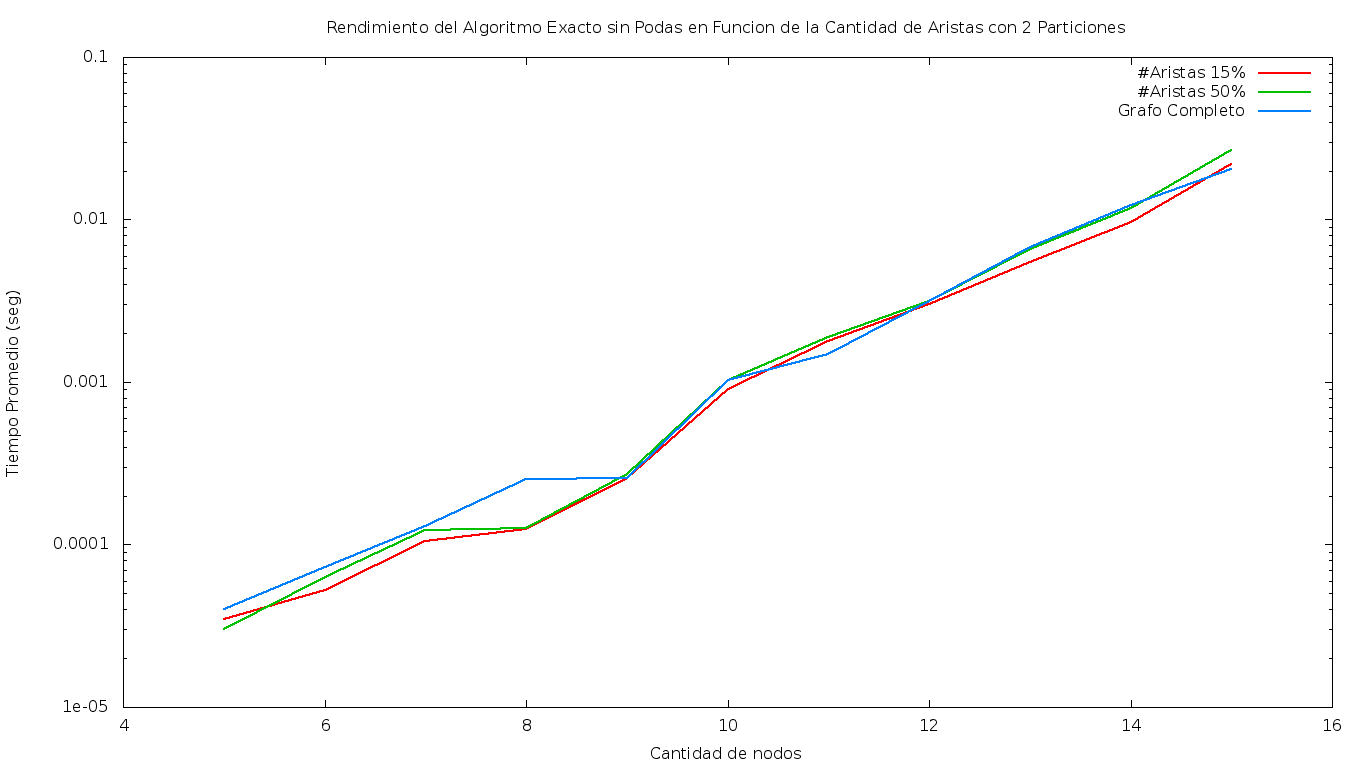
\includegraphics[scale=0.16]{finales/rendimientoExactoSinPoda2Particiones.png}
&
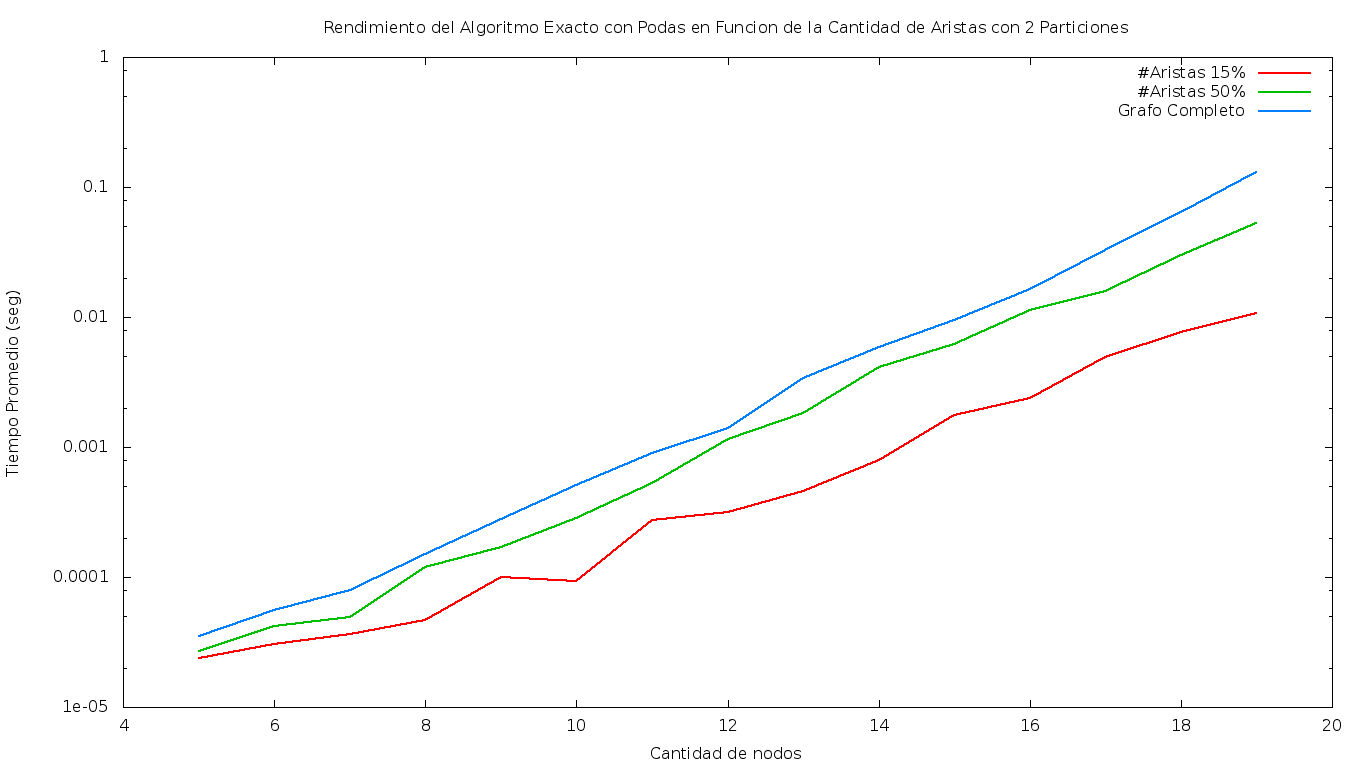
\includegraphics[scale=0.16]{finales/rendimientoExactoConPoda2Particiones.png}
\end{tabular}
\ec

\bc
\begin{tabular}{l c}
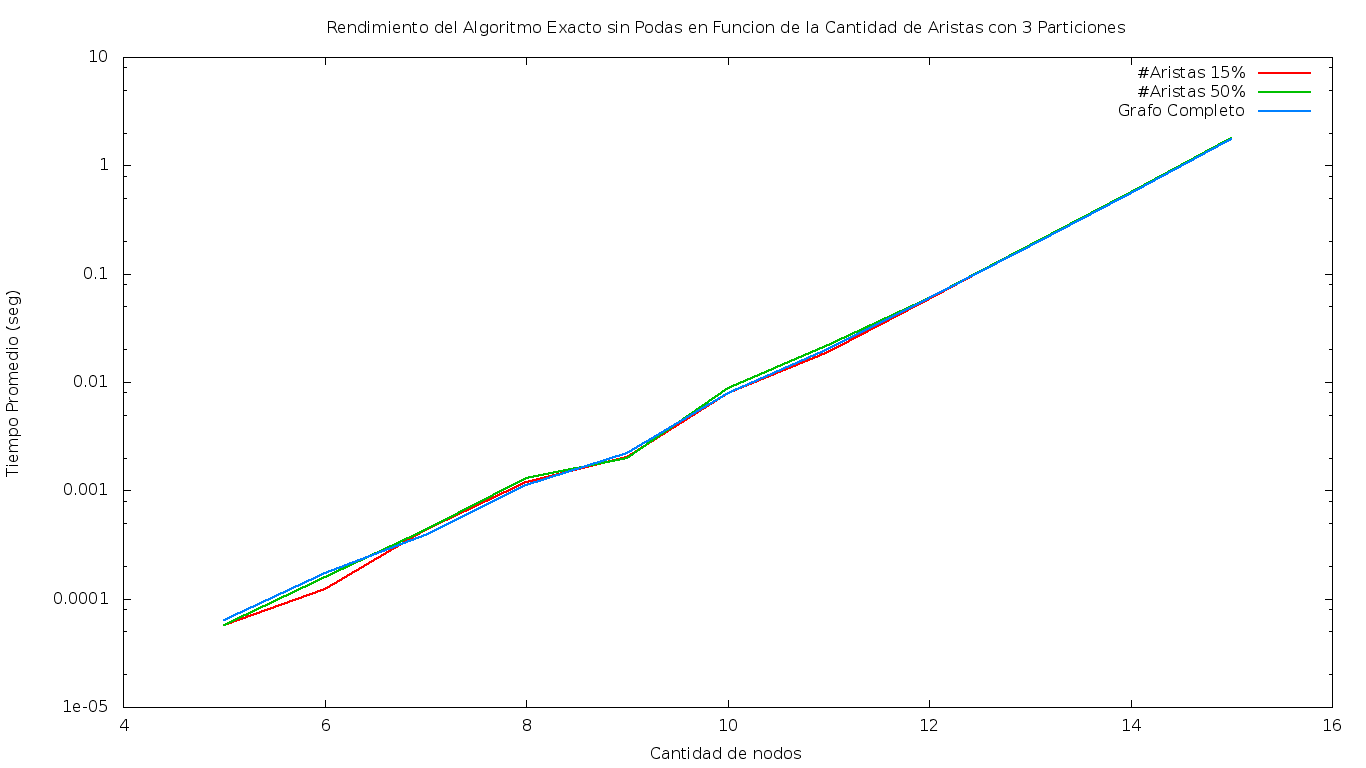
\includegraphics[scale=0.16]{finales/rendimientoExactoSinPoda3Particiones.png}
&
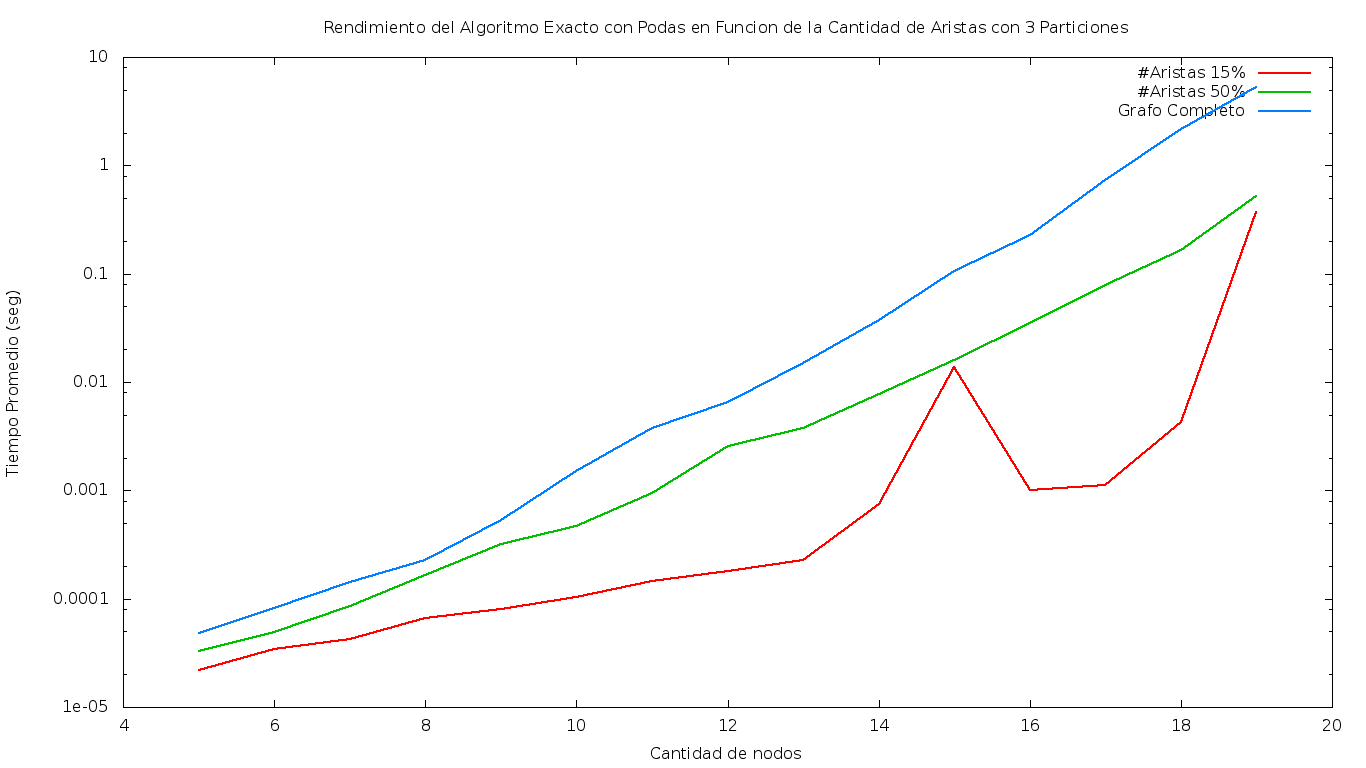
\includegraphics[scale=0.16]{finales/rendimientoExactoConPoda3Particiones.png}
\end{tabular}
\ec

\bc
\begin{tabular}{l c}
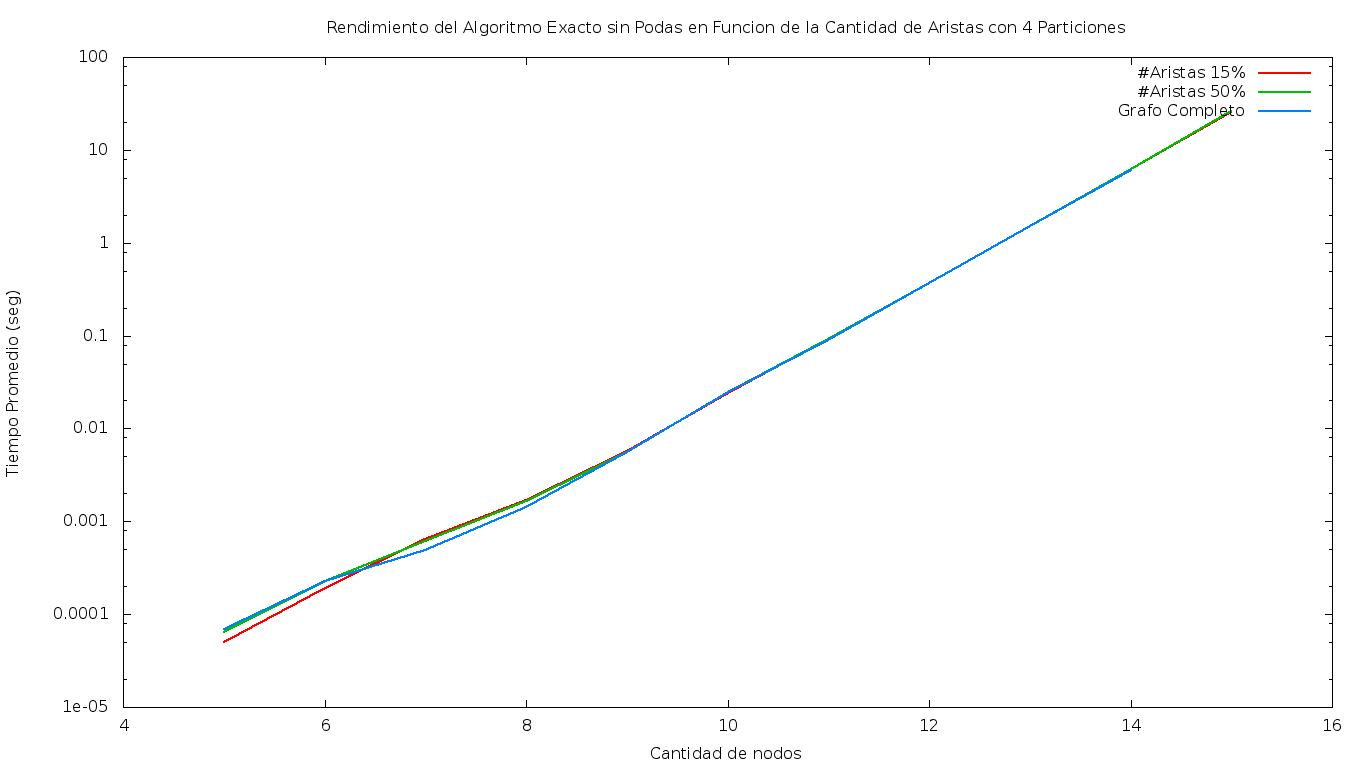
\includegraphics[scale=0.16]{finales/rendimientoExactoSinPoda4Particiones.png}
&
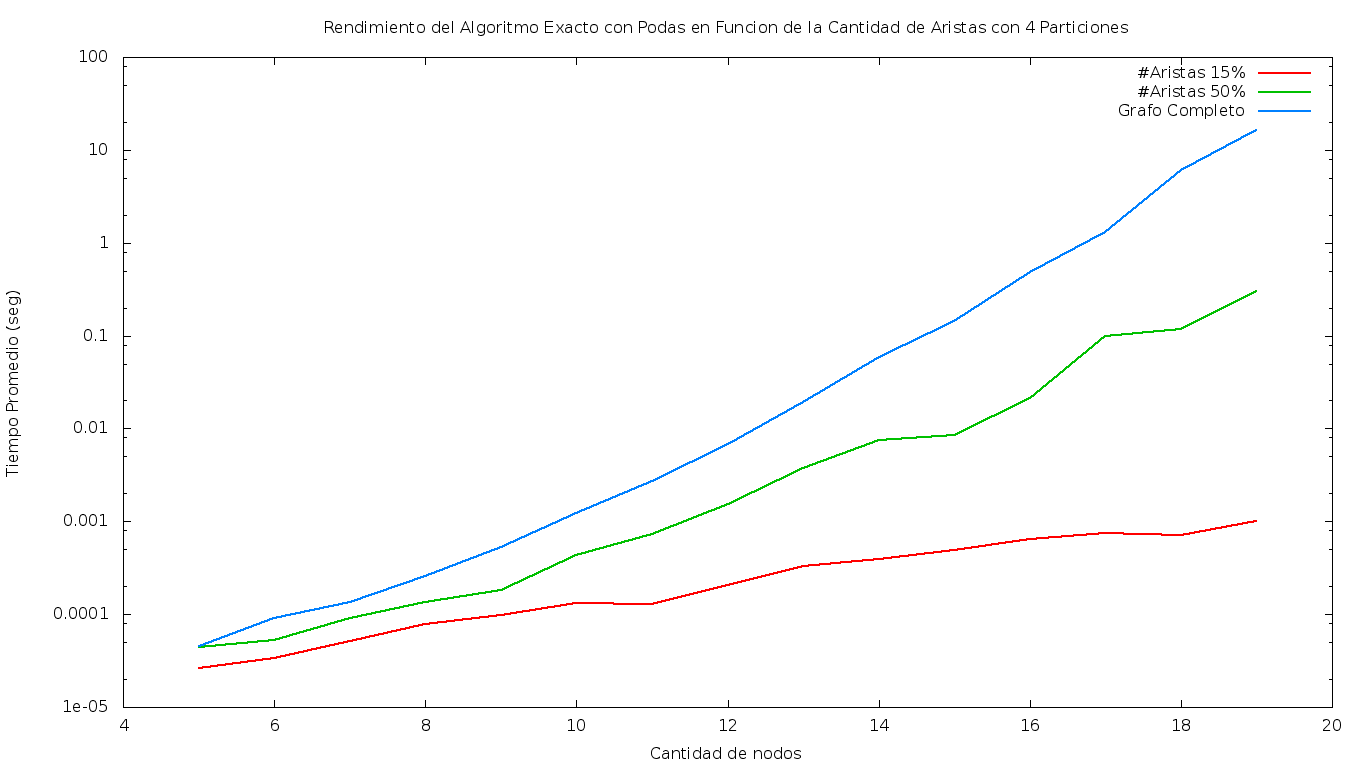
\includegraphics[scale=0.16]{finales/rendimientoExactoConPoda4Particiones.png}
\end{tabular}
\ec

\bc
\begin{tabular}{l c}
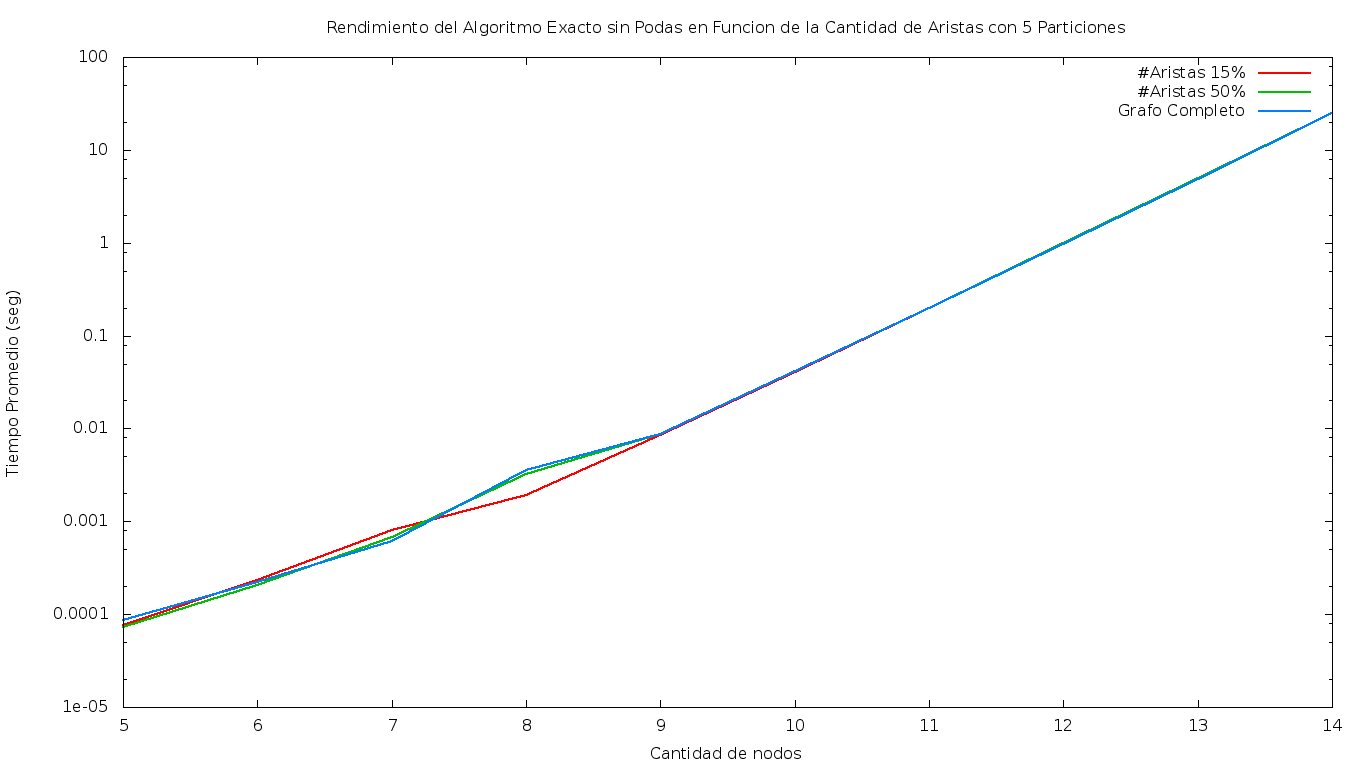
\includegraphics[scale=0.16]{finales/rendimientoExactoSinPoda5Particiones.png}
&
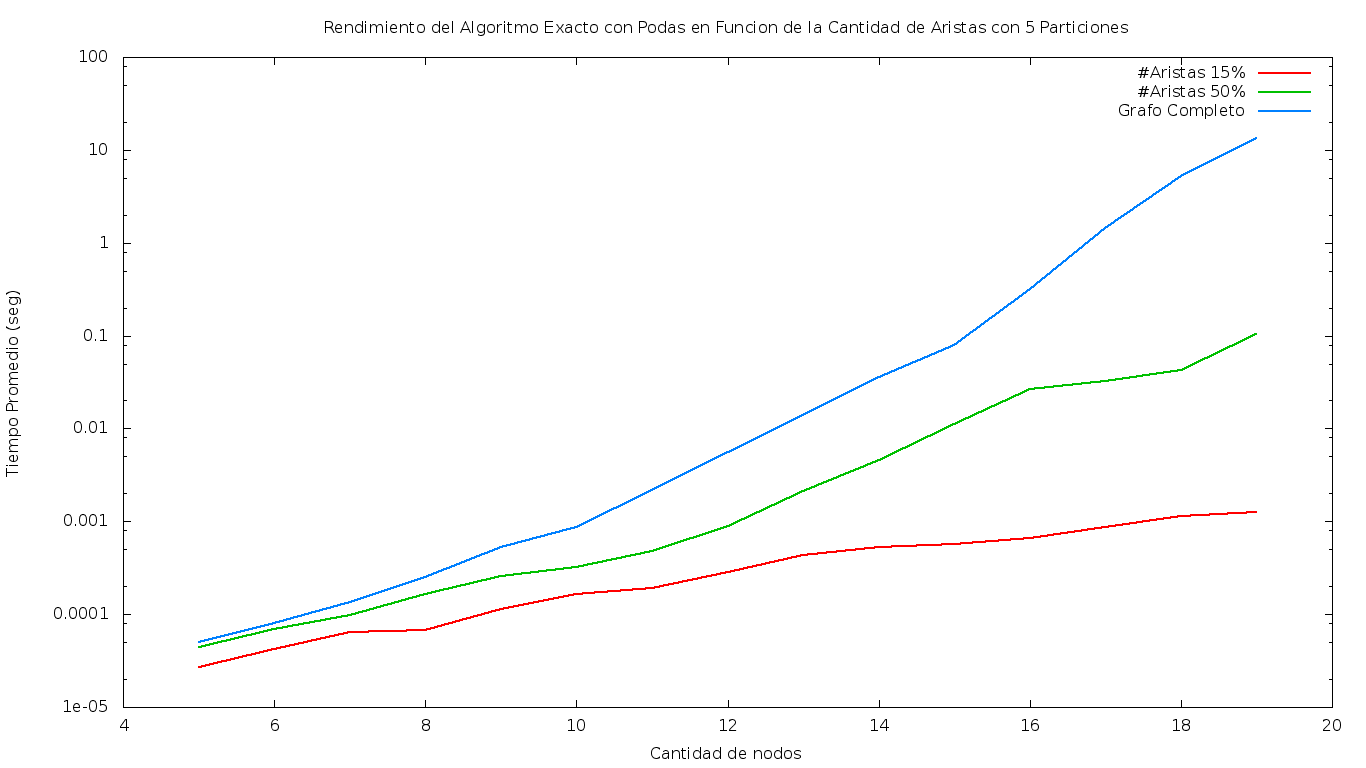
\includegraphics[scale=0.16]{finales/rendimientoExactoConPoda5Particiones.png}
\end{tabular}
\ec

\bc
\begin{tabular}{l c}
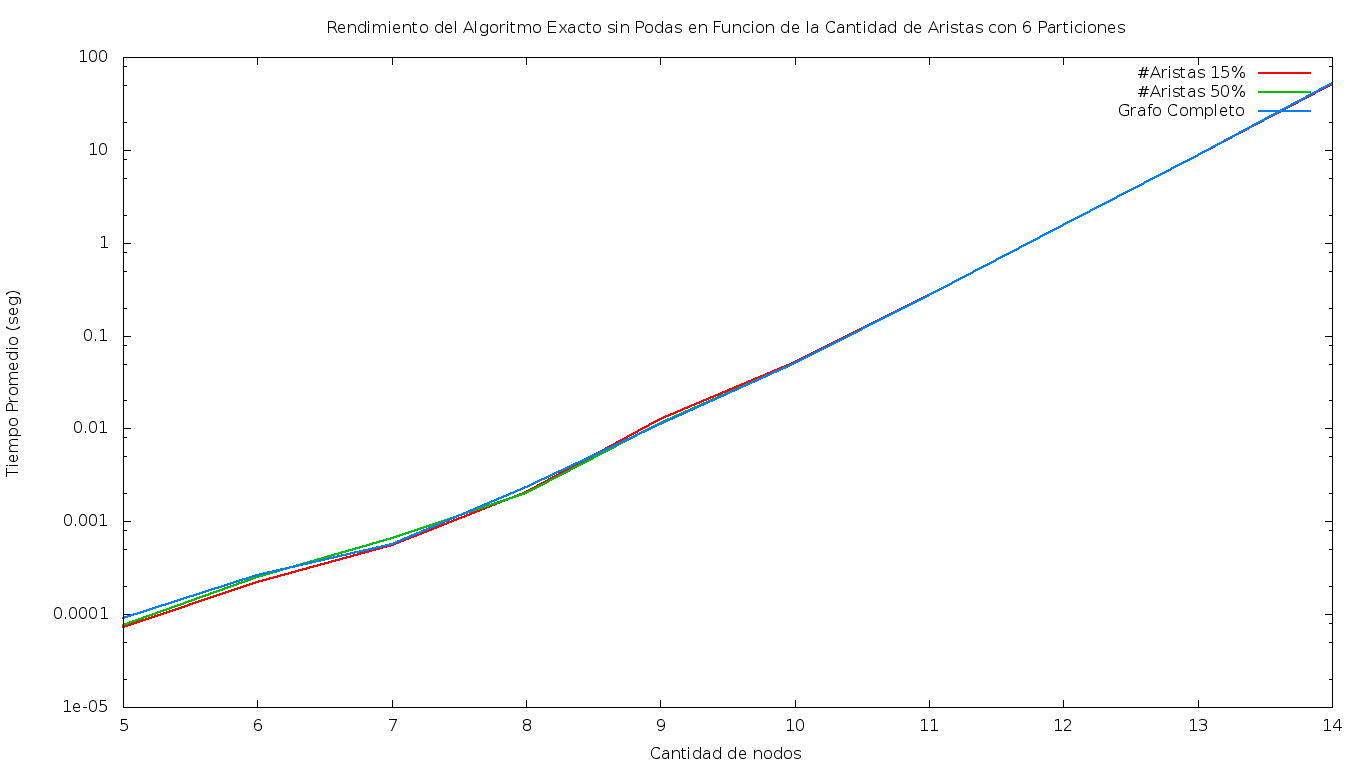
\includegraphics[scale=0.16]{finales/rendimientoExactoSinPoda6Particiones.png}
&
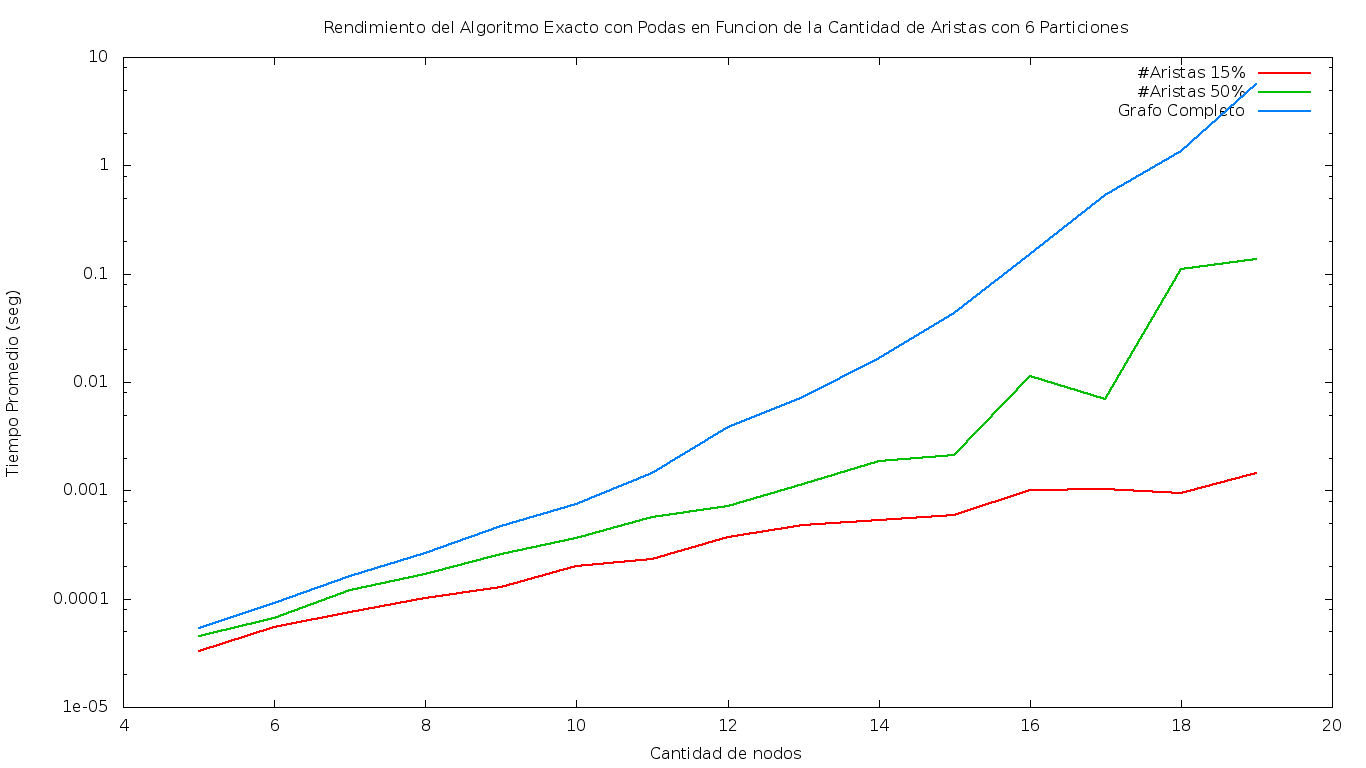
\includegraphics[scale=0.16]{finales/rendimientoExactoConPoda6Particiones.png}
\end{tabular}
\ec

\bc
\begin{tabular}{l c}
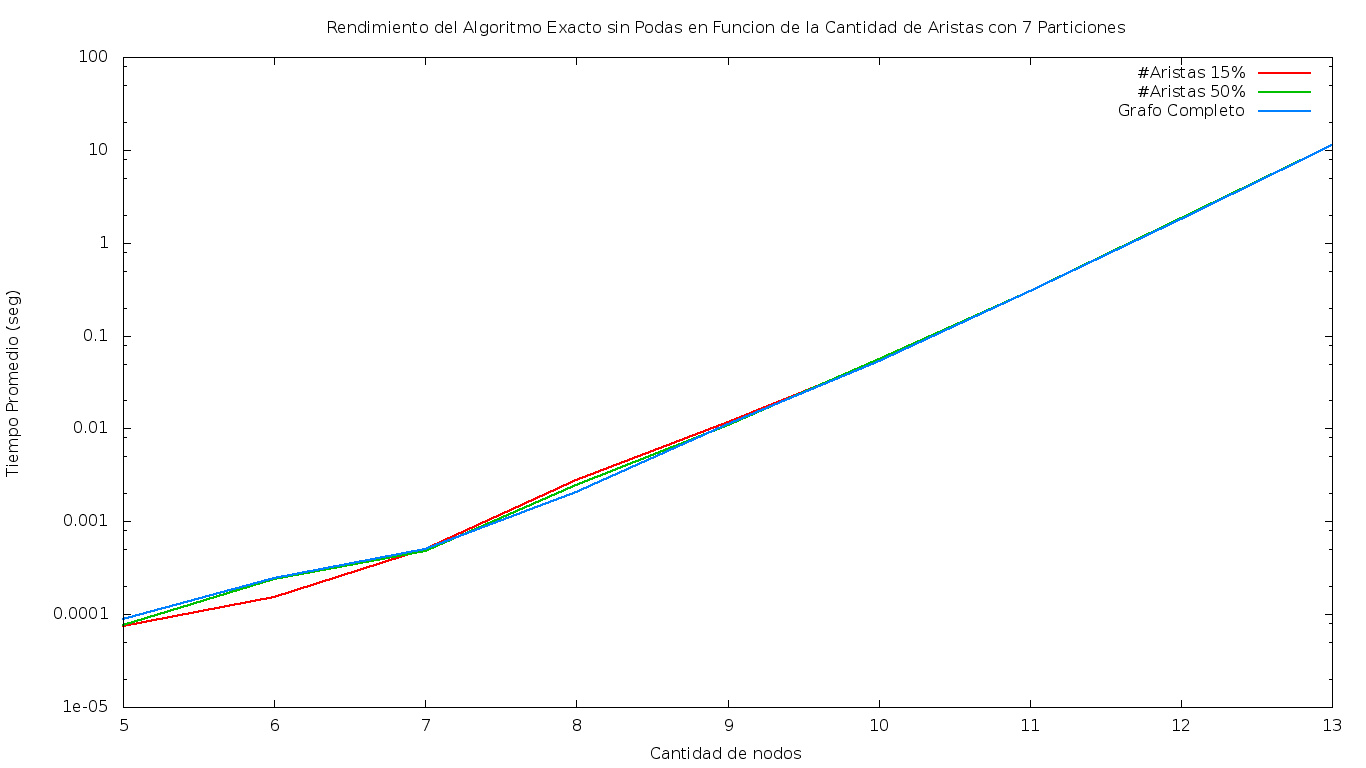
\includegraphics[scale=0.16]{finales/rendimientoExactoSinPoda7Particiones.png}
&
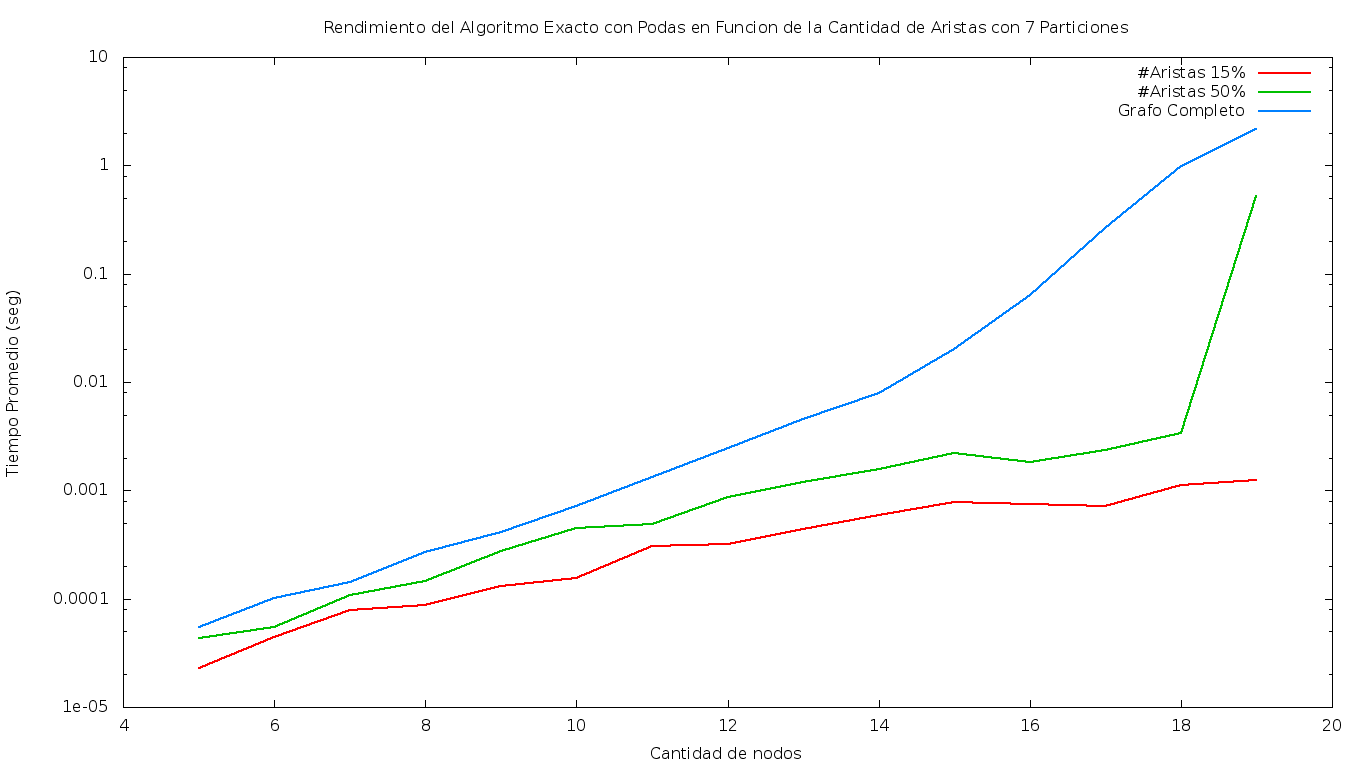
\includegraphics[scale=0.16]{finales/rendimientoExactoConPoda7Particiones.png}
\end{tabular}
\ec





\newpage
\section{Problema 3: La Comunidad del Anillo}
\subsection{Resoluci\'on}

Para nuestra heurística golosa comenzamos ordenando las aristas por peso de mayor a menor. Una vez obtenida la lista de aristas ordenadas por peso la iteramos escogiendo primero un nodo (arbitrariamente) de la arista más pesada y si la arista aun no se encuentra ubicada, se agrega a un nuevo conjunto siempre y cuando no hayamos sobrepasado la cantidad $k$ de conjuntos creados. En caso de que ya tengamos $k$ conjuntos o en caso de que hayamos terminado de recorrer las aristas se termina el ciclo.
Ahora verificamos si la cantidad de conjuntos creados es menor a $k$, en caso afirmativo habremos ubicado todos los nodos con aristas en alguno de los conjuntos.
Si quedan nodos sin ubicar, estos se agregan a cualquier conjunto, como ya agregamos todos los nodos de grado mayor a uno, los que restan se puede decir que tienen grado 0, por lo tanto, no importa en que conjunto sean agregados, estos no crearán aristas intraparticion y como consecuencia no sumarán peso a ningún conjunto.
Si la cantidad de conjuntos creados es igual a $k$, actuamos de forma diferente, aquí recorremos todas las aristas, actuando solo con las que no hayan sido agregadas a ningún conjunto de la siguiente manera: verificamos cuanto peso agregaría en cada conjunto para luego realmente añadirlo al conjunto que sume menos peso, en caso de encontrar uno en el que no cree aristas intraparticion, es agregado a este sin seguir revisando los restantes.

Como se puede observar usamos dos componentes greedys en la heurística:
La primera esta cuando se ordenan las aristas decrecientemente y se crean los $k$ conjuntos a medida que se separan los nodos de las aristas de mayor peso, para que estos no generen aristas intraparticion.
La segunda componente greedy se encuentra cuando al finalizar de crear los $k$ conjuntos se recorre nodo por nodo verificando si ya se encuentra agregado y en caso negativo, verificando en que conjunto genera menos peso para finalmente agregarlo a este.

A modo de ejemplo presentamos algunas imágenes para mostrar el funcionamiento de la heurística:

\begin{figure}[H]
\begin{center}
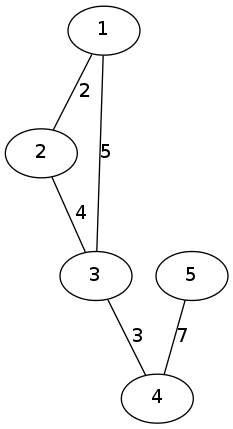
\includegraphics[scale=0.4]{./img/greedy1.png}
\caption{(1) Grafo de ejemplo}
\end{center}
\end{figure}
La primer imagen corresponde al grafo al que se le aplicará k-PMP (1)

\begin{figure}[H]
\begin{center}
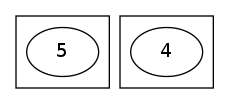
\includegraphics[scale=0.4]{./img/greedy2.png}
\caption{(2) Conjuntos 1 y 2 luego de separar los nodos de las aristas mas pesadas}
\end{center}
\end{figure}
Luego de ordenar las aristas escoge las de mayor tamaño y separa sus nodos en k conjuntos k=2 para este ejemplo. (2)

\begin{figure}[H]
\begin{center}
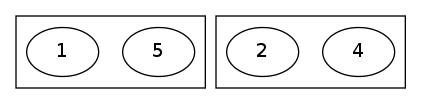
\includegraphics[scale=0.4]{./img/greedy3.png}
\caption{(3) Conjuntos luego de comenzar a ingresar los nodos restantes}
\end{center}
\end{figure}
Luego como ya hay 2 conjuntos creados procede a verificar nodo los nodos y agregándolos al conjunto que menos sume. En el caso del nodo 1, se agrega de inmediato al primer conjunto porque no genera arista intraparticion. Para el nodo 2 primero verifica en el 1er conjunto, aquí sumaria 2 de peso, se verifica en el siguiente conjunto, y como no suma peso, se ingresa ahí. (3)

\begin{figure}[H]
\begin{center}
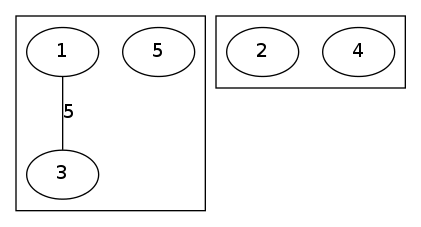
\includegraphics[scale=0.4]{./img/greedy4.png}
\caption{(4) Resultado de haber corrido la heurística greedy al grafo (1)}
\end{center}
\end{figure}
Finalmente resta agregar el nodo 3 el cual genera en el conjunto uno un peso igual a 5, y en el conjunto 2 un peso igual a 7 al unirse con los nodos 2 y 4. Por lo tanto el nodo 3 es introducido en el conjunto 1. (4)


A continuación presentamos un pseudo-gráfico del algoritmo
\begin{itemize}
\item ordenar $aristas$ por peso en orden decreciente
\item mientras restan $aristas$ 
  \begin{itemize}
  \item si no hay $k$ conjuntos, crear conjunto y agregar $nodo1$ de $arista$ (si este no pertenece a ningún conjunto)
  \item sino cortar el ciclo  
  \item si no hay $k$ conjuntos, crear conjunto y agregar $nodo2$ de $arista$ (si este no pertenece a ningún conjunto)
  \item sino cortar el ciclo  
  \end{itemize}
\item Si hay menos de $k$ conjuntos creados
  \begin{itemize}
  \item agregar las aristas que quedaron fuera a alguno de los conjuntos creados
  \end{itemize}
\item Sino
  \begin{itemize}
  \item desde nodo 0 a nodo n-1
    \begin{itemize}
    \item si el nodo no esta en ningún conjunto
      \begin{itemize}
        \item verificar conjunto por conjunto cuanto peso generaría agregarlo a este
        \item agregar el nodo al conjunto en el que genere menos peso
      \end{itemize}
    \end{itemize}
  \end{itemize}
\end{itemize}




\subsection{Análisis de complejidad}

Vamos a analizar el código paso por paso analizando la complejidad temporal del peor caso.
Lo primero que hacemos es ordenar las aristas, para esto utilizamos la función $sort$ de la $std$ que posee una complejidad temporal de $O(n.log(n))$, en este caso como se aplica a las aristas esto es $O(m.log(m))$ siendo $m$ la cantidad de aristas.
A continuación, y haciendo uso del pseudocódigo proporcionado:
\begin{itemize}
\item mientras restan $aristas$ 
  \begin{itemize}
  \item si no hay $k$ conjuntos, crear conjunto y agregar $nodo1$ de $arista$ (si este no pertenece a ningún conjunto)
  \item sino cortar el ciclo  
  \item si no hay $k$ conjuntos, crear conjunto y agregar $nodo2$ de $arista$ (si este no pertenece a ningún conjunto)
  \item sino cortar el ciclo  
  \end{itemize}
\end{itemize}
Este scope tiene una complejidad $O(m)$ ya que se recorren todas las aristas, en el peor caso creando conjuntos y agregándolos a estos, pero estas dos acciones tienen una complejidad constante.

A continuación si se crearon menos de $k$ conjuntos se agregan los nodos que restan a uno de estos. En el peor caso esto pertenece al orden de $O(n)$ siendo n la cantidad de nodos.
Si hay $k$ conjuntos creados se procede de la siguiente manera:
\begin{itemize}
\item desde nodo 0 a nodo n-1   $O(n)$
  \begin{itemize}
  \item si el nodo no esta en ningún conjunto $O(1)$
    \begin{itemize}
      \item verificar conjunto por conjunto cuanto peso generaría agregarlo a este $O(k+n)$
      \item agregar el nodo al conjunto en el que genere menos peso $O(1)$
    \end{itemize}
  \end{itemize}
\end{itemize}

Esta ultima parte del algoritmo tiene una complejidad acotada en el peor caso de O($n^{2}$) ya que por cada nodo no agregado ($n$ en total en el peor caso) se verifica cuanto pesaría agregarlo a cada conjunto. Para esto se recorren los nodos ya ingresados en el conjunto actual (peor caso $n$) y se agrega al que menor peso aporte. Esto tiene relación con el $k$ también ya que en el peor caso se verificará en los $k$ conjuntos.

\subsection{Instancias desfavorables}


Probamos la heurística con varias familias de grafos, grafos estrella...(ETC) 
Para el caso de los grafos estrella nuestra heurística funcionaba mal, particularmente cuando el numero del nodo central era superior a la cantidad k de conjuntos. 
Para aclarar, en un principio nuestro algoritmo constaba solo de la segunda componente greedy de la que se habla en la sección Resolución. Por lo que comenzaba desde el primer nodo hasta el ultimo probando en que conjunto convenía poner dicho nodo de forma de disminuir lo mas posible el peso total de las aristas intraparticion. Volviendo al caso del grafo estrella, lo que pasaba era que ingresaba en los

\subsection{Experimentación}

Para poder observar la performance del algoritmo en términos de tiempo de ejecución en función al tamaño de la entrada nos construimos un script en python que genera tres tipos de grafos, grafos con un 15 \% de aristas, uno con un 50 \% de aristas y el último con el 100 \% de aristas, tomando para el porcentaje la cantidad de aristas que llevaría un grafo completo.
Para cada uno de estos variamos los valores de n y de k con n entre 100 y 500. 
Por cada uno de esos valores de n, variamos el valor de k entre 2 y 10.
Cada una de todas estas instancias fueron corridas entre 20 y 30 veces, (20 para las instancias mas grandes) para poder calcular un promedio. Ya que consideramos que el procesador no esta ejecutando solo nuestra heurística, por lo que el tiempo que le toma correr el algoritmo hasta obtener una solución seguramente es mayor al real. Por otro lado también pensamos en la posibilidad de que el procesador cachee las soluciones al estar haciendo muchas veces lo mismo, razón por la cual decidimos no superar las 30 repeticiones. Entre estas dos cosas donde una desfavorece y otra favorece el tiempo de ejecución, nos pareció razonable realizar un promedio.
Con los valores obtenidos presentamos algunos gráficos para tener una descripción mas visual y los analizamos.

\begin{figure}[H]
\begin{center}
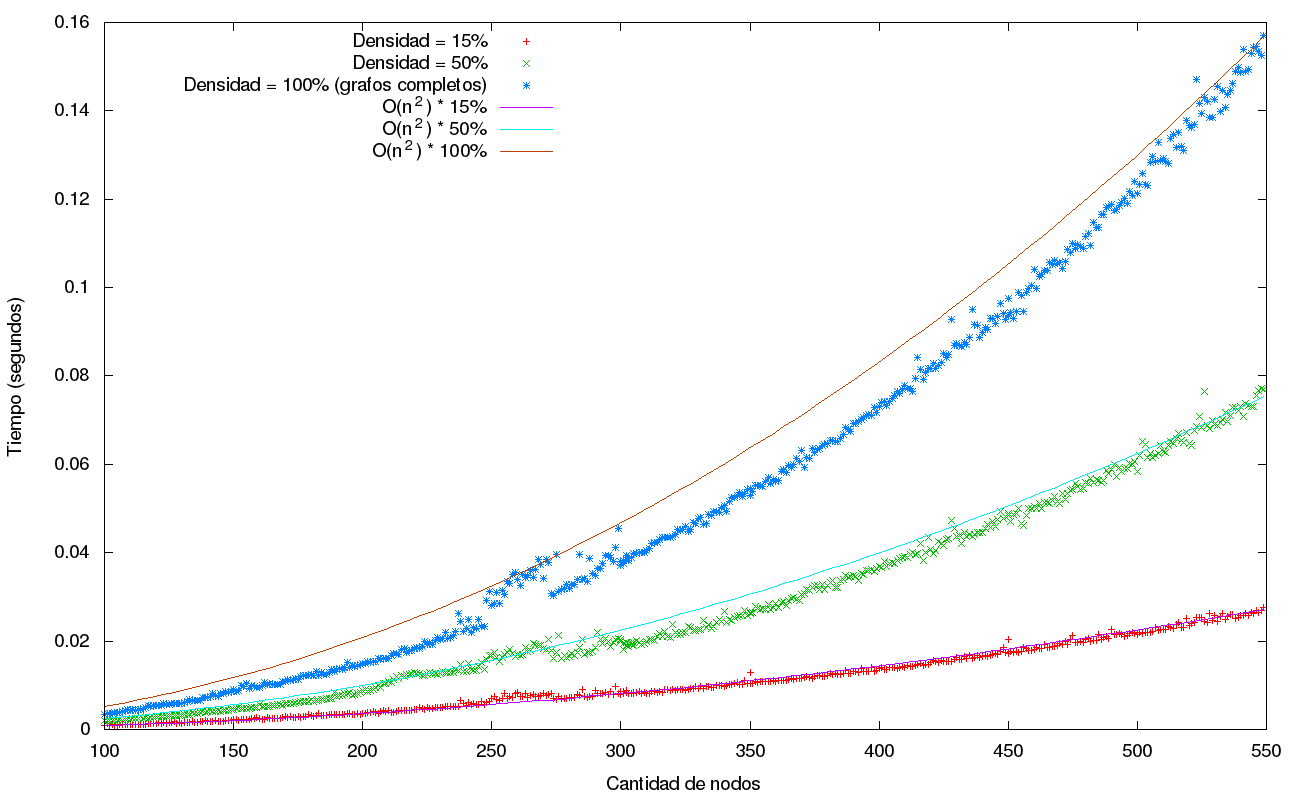
\includegraphics[scale=0.4]{./img/greedyN1.png}
\caption{Gráficos con k = 2}
\end{center}
\end{figure}

\begin{figure}[H]
\begin{center}
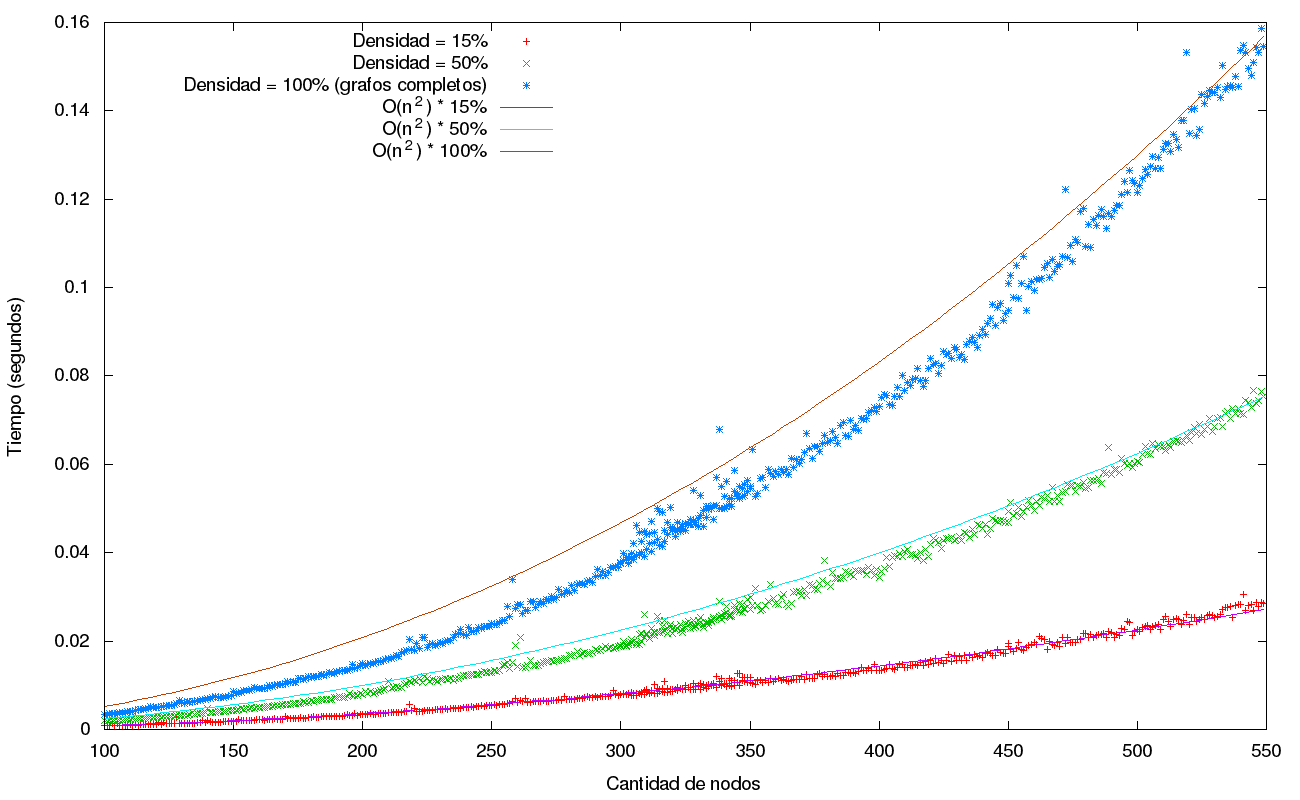
\includegraphics[scale=0.4]{./img/greedyN2.png}
\caption{Gráficos con k = 5}
\end{center}
\end{figure}

\begin{figure}[H]
\begin{center}
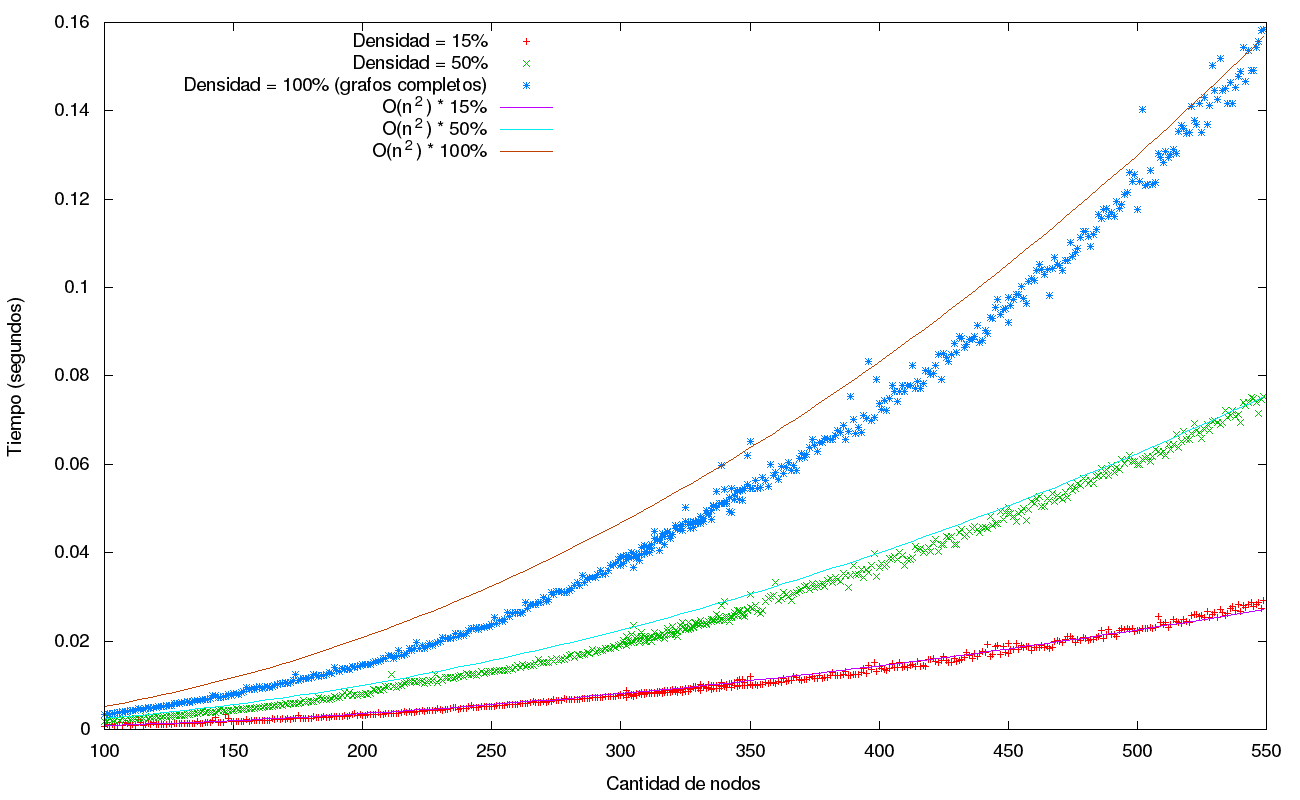
\includegraphics[scale=0.4]{./img/greedyN3.png}
\caption{Gráficos con k = 10}
\end{center}
\end{figure}


En estos gráficos podemos observar que el algoritmo tiene una complejidad de $n^{2}$ en relación a la cantidad de nodos, la cual obviamente se ve afectada al mismo tiempo por la cantidad de aristas que el grafo posee. Esta observación se puede notar ya que cada grafo presenta la complejidad temporal para una densidad de aristas de 15\%, 50\% y 100\% comparada con un valor $n^{2}$ multiplicado por una constante obtenida a partir de dividir el tiempo sobre la cantidad de nodos, y a su vez este valor es multiplicado por 0.15, 0.50 y 1.
Al hacer esto y verificar que los valores se asemejan demasiado podemos concluir que la cantidad de aristas del grafo afecta directamente al rendimiento de forma lineal.

En los tres gráficos utilizamos los mismos valores para O($n^{2}$)* densidad de cantidad de aristas, y como se puede observar comparando los distintos gráficos, que presentan una variación en la cantidad k de conjuntos, los valores resultantes de los tests son casi los mismos, no se nota ninguna variación apreciable. 



%\begin{figure}[H]
%\begin{center}
%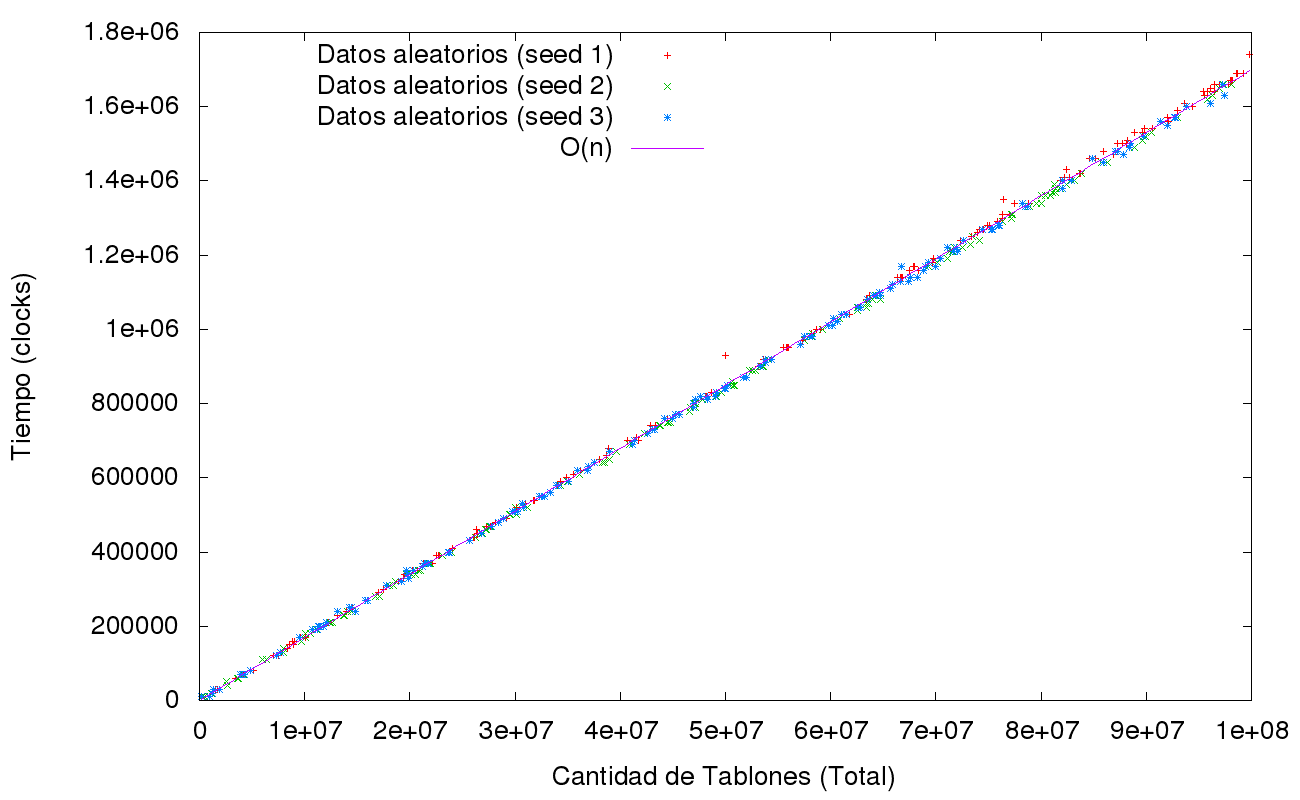
\includegraphics[scale=0.4]{./imágenes/ej1_chartRendimiento.png}
%\caption{Gr\'afico de tiempos con test pseudo-aleatorios.}
%\end{center}
%end{figure}



\newpage
\begin{thebibliography}{2}

\bibitem{sort}
  C++ reference,
  \url{http://www.cplusplus.com/reference/algorithm/sort/}
 

\bibitem{upper}
	C++ reference,
	\url{http://www.cplusplus.com/reference/map/multimap/}
  
\end{thebibliography}



\end{document}

\end{document}
